\section{建立子路径}
\subsection{简述建立子路径}
MPTCP在进行三次握手之后,客户端和服务端会进行地址信息的交换,让对方知道彼此未用的地址信息。当客户端知道服务端的地址后就可以建立其他子路径。三次握手和建立子路径的过程如下图:
\begin{figure}[H]
  \centering
  % Requires \usepackage{graphicx}
  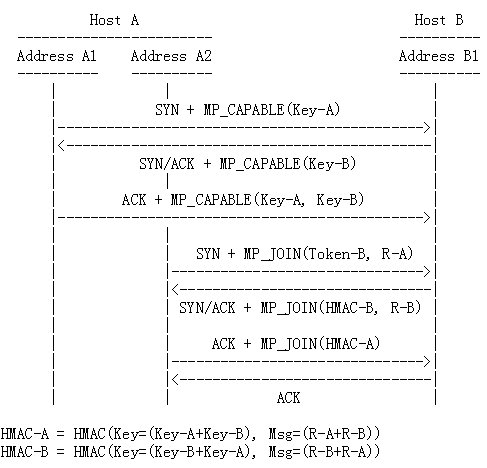
\includegraphics[width=8cm]{dias/Create_Subflows.jpg}\\
  \caption{建立子路径}
\end{figure}

关于Token、随机数R、以及HMAC(Hash-based Message Authentication Code)的详细解释可以阅读参考:\verb|https://tools.ietf.org/html/rfc6824#section-3.2|。

\subsection{建立子路径的内核实现}
这里我们主要关注建立子路径过程中,master sock对slave sock的影响。当客户端发送第一个SYN准备建立子路径的时候就会调用mptcp\_init4\_subsockets来创建一个新的socket和相应的sock。
\small\begin{verbatim}
"net/mptcp/mptcp_ipv4.c" line 328 of 488
328 int mptcp_init4_subsockets(struct sock *meta_sk, const struct mptcp_loc4 *loc,
329                struct mptcp_rem4 *rem)
330 {
331     struct tcp_sock *tp;
332     struct sock *sk;
333     struct sockaddr_in loc_in, rem_in;
334     struct socket sock;
335     int ulid_size = 0, ret;
336
337     /** First, create and prepare the new socket */
338
339     sock.type = meta_sk->sk_socket->type;
340     sock.state = SS_UNCONNECTED;
341     sock.wq = meta_sk->sk_socket->wq;
342     sock.file = meta_sk->sk_socket->file;
343     sock.ops = NULL;
344
345     ret = inet_create(sock_net(meta_sk), &sock, IPPROTO_TCP, 1);
346     if (unlikely(ret < 0)) {
347         mptcp_debug("%s inet_create failed ret: %d\n", __func__, ret);
348         return ret;
349     }
350
351     sk = sock.sk;
352     tp = tcp_sk(sk);
\end{verbatim}\normalsize
第345行的函数inet\_create创建了子路径的socket和sock。
\small\begin{verbatim}
354     /* All subsockets need the MPTCP-lock-class */
355     lockdep_set_class_and_name(&(sk)->sk_lock.slock, &meta_slock_key, "slock-AF_INET-MPTCP");
356     lockdep_init_map(&(sk)->sk_lock.dep_map, "sk_lock-AF_INET-MPTCP", &meta_key, 0);
357
358     if (mptcp_add_sock(meta_sk, sk, loc->loc4_id, rem->rem4_id, GFP_KERNEL))
359         goto error;
360
361     tp->mptcp->slave_sk = 1;
362     tp->mptcp->low_prio = loc->low_prio;
363
364     /* Initializing the timer for an MPTCP subflow */
365     setup_timer(&tp->mptcp->mptcp_ack_timer, mptcp_ack_handler, (unsigned long)sk);
\end{verbatim}\normalsize
第358行的mptcp\_add\_sock将master sock 和 子路径的sock联系起来。第361行表面此sock为 slave subsock。\\
第362行设置此子路径是否为备用路径。只有现在路径都不可用的情况下,才会通过备用子路径发送数据。\\
第365行设置的定时器用于重发建立子路径的最后一个ACK,这样做是为了保证上图中的HMAC-A可以送达。
\small\begin{verbatim}
369     ulid_size = sizeof(struct sockaddr_in);
370     loc_in.sin_family = AF_INET;
371     rem_in.sin_family = AF_INET;
372     loc_in.sin_port = 0;
373     if (rem->port)
374         rem_in.sin_port = rem->port;
375     else
376         rem_in.sin_port = inet_sk(meta_sk)->inet_dport;
377     loc_in.sin_addr = loc->addr;
378     rem_in.sin_addr = rem->addr;
379
380     ret = sock.ops->bind(&sock, (struct sockaddr *)&loc_in, ulid_size);
381     if (ret < 0) {
382         mptcp_debug("%s: MPTCP subsocket bind() failed, error %d\n",
383                 __func__, ret);
384         goto error;
385     }
386
387     mptcp_debug("%s: token %#x pi %d src_addr:%pI4:%d dst_addr:%pI4:%d\n",
388             __func__, tcp_sk(meta_sk)->mpcb->mptcp_loc_token,
389             tp->mptcp->path_index, &loc_in.sin_addr,
390             ntohs(loc_in.sin_port), &rem_in.sin_addr,
391             ntohs(rem_in.sin_port));
392
393     if (tcp_sk(meta_sk)->mpcb->pm_ops->init_subsocket_v4)
394         tcp_sk(meta_sk)->mpcb->pm_ops->init_subsocket_v4(sk, rem->addr);
395
396     ret = sock.ops->connect(&sock, (struct sockaddr *)&rem_in,
397                 ulid_size, O_NONBLOCK);
398     if (ret < 0 && ret != -EINPROGRESS) {
399         mptcp_debug("%s: MPTCP subsocket connect() failed, error %d\n",
400                 __func__, ret);
401         goto error;
402     }
\end{verbatim}\normalsize
第380行是将子路径的socket的与地址绑定。第396行此套接字将会调用tcp\_v4\_connect进行连接操作。
\small\begin{verbatim}
404     sk_set_socket(sk, meta_sk->sk_socket);
405     sk->sk_wq = meta_sk->sk_wq;
406
407     return 0;
408
409 error:
410     /* May happen if mptcp_add_sock fails first */
411     if (!mptcp(tp)) {
412         tcp_close(sk, 0);
413     } else {
414         local_bh_disable();
415         mptcp_sub_force_close(sk);
416         local_bh_enable();
417     }
418     return ret;
419 }
\end{verbatim}\normalsize
第404和405行将子路径的sk和master的socket建立联系,因为对于应用程序来说只有master的socket是可见,而slave subsock的socket是不可见。下面的情景是服务端收到上图:Figure 5 中ACK/MP\_JOIN(HMAC-A)包,这时状态将由SYN\_RECV变为ESTABLISHED。函数的调用
关系如下:
\small\begin{verbatim}
tcp_v4_rcv
          =》tcp_v4_do_rcv
               =》mptcp_v4_do_rcv
                    =》tcp_v4_hnd_req
                         =》tcp_check_req
                              =》mptcp_check_req_child
                                    =》mptcp_add_sock
\end{verbatim}\normalsize

在函数tcp\_check\_req中将会建立新的sock。主要代码如下:
\small\begin{verbatim}
"net/ipv4/tcp_minisocks.c" line 766 of 872
760     /* OK, ACK is valid, create big socket and
761      * feed this segment to it. It will repeat all
762      * the tests. THIS SEGMENT MUST MOVE SOCKET TO
763      * ESTABLISHED STATE. If it will be dropped after
764      * socket is created, wait for troubles.
765      */
766 #ifdef CONFIG_MPTCP
767     if (mptcp(tcp_sk(sk)))
768         /* MPTCP: We call the mptcp-specific syn_recv_sock */
769         child = tcp_sk(sk)->mpcb->syn_recv_sock(sk, skb, req, NULL);
770     else
771 #endif
772         child = inet_csk(sk)->icsk_af_ops->syn_recv_sock(sk, skb,
773                 req, NULL);
774
775     if (child == NULL)
776         goto listen_overflow;
\end{verbatim}\normalsize
第769行将会调用mptcp\_syn\_recv\_sock和tcp\_v4\_syn\_recv\_sock和tcp\_create\_openreq\_child创建新的sock并进行初始化。函数mptcp\_check\_req\_child和mptcp\_add\_sock会将此sock 和master sock建立联系,并且设置此sock的属性slave\_sk为1.
\subsection{结论}
\begin{itemize}
  \item MPTCP利用Token、随机数R、以及HMAC(Hash-based Message Authentication Code)这些信息的交换保证构建子路径正确。
  \item sub sock是在meta sock基础上建立,只有meta对于应用层是可见,其余sub sock并不可见。
\end{itemize}